The thermal network consists of heat sources (some of which are temperature-dependent) and thermal resistances. The latter are given by the properties of the mechanical design (heat conductivities of the materials) and the geometry of the heat path. The geometry is generally 3-dimensional, but it is the strategy of the simple network models to lump the 3D behaviour into one thermal resistance parameter. In the models discussed here, we have used a granularity corresponding to single detector modules for which the thermal resistance has been modelled. The temperatures in the model are then given for the nodes in the network in analogy to the potentials in an electrical network.

The complexity of the thermal network used in this study, depicted in Fig.~\ref{fig:thermalmodel}, is given by the variety of temperature-dependent heat sources in the ATLAS strip system: the digital power for each type of chip, the FEAST chip providing the on-detector DC-DC conversion, and the sensor leakage power. In the ATLAS ITk strip modules, all of these components are located on top of the sensors, such that the heat generated in them flows through the sensor into the support structure, the stave (barrel) or petal (endcap) core with the embedded cooling pipe. In the network model, the heat flow from these sources combines and travels through a common impedance $R_\text{M}$ to the sink at a temperature $T_\text{C}$. For each of the temperature-dependent heat sources (ABC, HCC, FEAST and the sensor) we have added a resistance from the common temperature $T_\text{mod}$ to allow for a finite and different heat path for each of them. Finally, the EOS card adjacent to the last module on the barrel stave or endcap petal is modeled as an additional source of heat with an independent impedance for its unique thermal path.

\begin{figure}[ht]
\centering
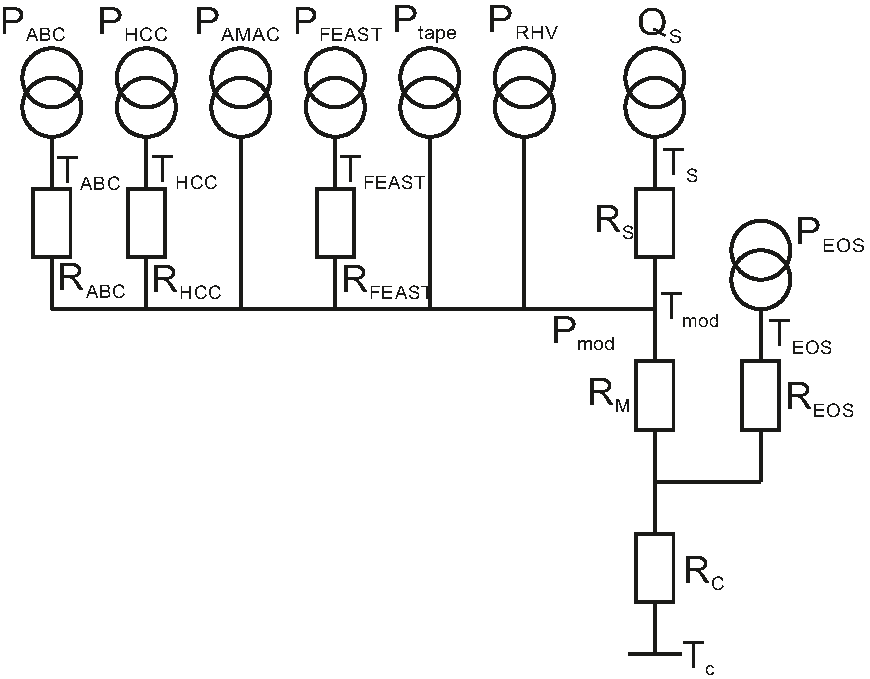
\includegraphics[width=0.6\linewidth]{figures/Thermalmodel.pdf}
\caption{Thermal network model.}
\label{fig:thermalmodel}
\end{figure}

This is a more complex thermal network than the one studied in Ref.~\cite{Beck:2010zzd}, for which an analytical solution for the determination of thermal stability is given. In particular, because of the non-linear temperature dependence of some of the heat sources, it is not possible in the present case to solve the set of equations describing the model analytically. However, the set of equations is still sufficiently small to solve numerically using any modern programming language.
